
\documentclass[a4paper,10pt,article,oneside,english]{memoir} 
% DANSK OPSÆTNING
\usepackage[english]{babel}
\usepackage[utf8]{inputenc}
\usepackage[T1]{fontenc}
\usepackage{lmodern} 
\renewcommand{\englishhyphenmins}{22} 


% FIGURER
\usepackage{graphicx}

% MATEMATIK
\usepackage{amsmath}
\usepackage{amssymb,amsthm,bm}
\usepackage{mathtools}	


% This document uses
\usepackage[draft,silent]{fixme}
\usepackage{hyperref}
\usepackage{siunitx}


% captions in italic
\let\oldcaption\caption
\renewcommand{\caption}[1]{\oldcaption{\emph{#1}}}


\begin{document}
	%\frontmatter
	%\clearpage	
	%\tableofcontents*
	\title{Machine Learning E16 - Handin 3\\
		 Hidden Markov Model for Gene Finding in Prokaryotes}
	\author{Group 22\\
		Mark Medum Bundgaard, Morten Jensen, Martin Sand Nielsen}
	\date{\today, Aarhus University}
	
	\mainmatter
	\maketitle
	
\begin{figure}
	\centering
	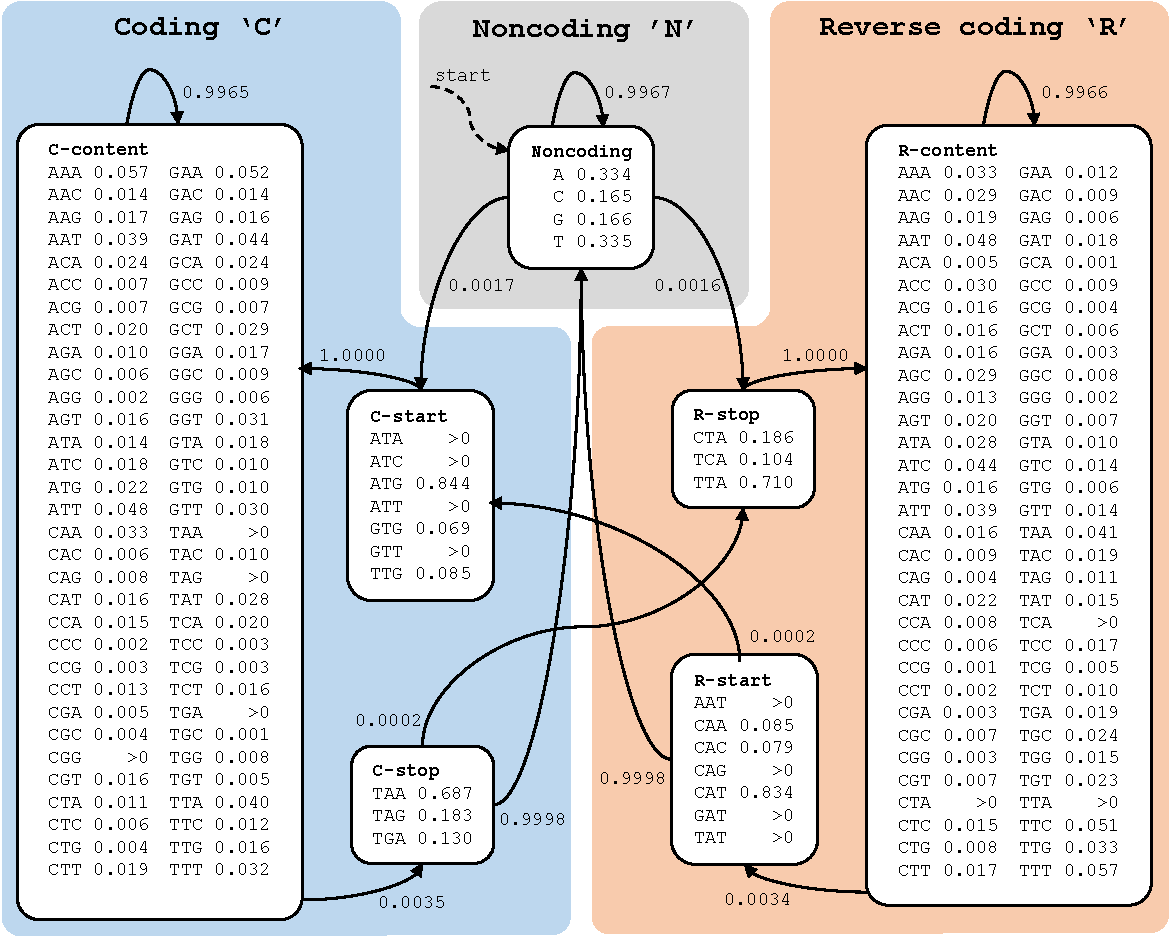
\includegraphics[width=\linewidth]{HMM_graph_cropped.pdf}
	\caption{State graph for out HMM for genome annotation by explicitly matching codons within coding areas, and enforcing certain start and stop codons. Transition and emission probabilities gained by counting annotated data.}
	\label{fig:hmm_graph}
\end{figure}
	
	
\end{document}
